% Chapter 1

\chapter{Introducción General} % Main chapter title

\label{Chapter1} % For referencing the chapter elsewhere, use \ref{Chapter1} 
\label{IntroGeneral}

%----------------------------------------------------------------------------------------

% Define some commands to keep the formatting separated from the content 
\newcommand{\keyword}[1]{\textbf{#1}}
\newcommand{\tabhead}[1]{\textbf{#1}}
\newcommand{\code}[1]{\texttt{#1}}
\newcommand{\file}[1]{\texttt{\bfseries#1}}
\newcommand{\option}[1]{\texttt{\itshape#1}}
\newcommand{\grados}{$^{\circ}$}

%----------------------------------------------------------------------------------------

En este capítulo se introduce brevemente el campo de la acústica submarina y la importancia del parámetro SONAR Ruido Ambiente Submarino como motivación para la realización de este trabajo.  Se presentan los objetivos y el alcance del proyecto.
%----------------------------------------------------------------------------------------
\section{Descripción técnica-conceptual del proyecto}

%Contexto que da origen al proyecto de investigación.
%Introducción conceptos de acústica submarina.
%Qué es el ruido submarino.
%Cómo se mide / intro hidrófono.

La acústica submarina estudia la propagación del sonido en el agua y la interacción de las ondas mecánicas que constituyen el sonido con el agua, los elementos dispersores presentes y las interfaces aire-agua y agua-lecho marino.  Debido a que sufre menor atenuación que otras formas de radiación, el sonido es ampliamente empleado  por el hombre en su exploración de los océanos.  Las frecuencias típicas utilizadas se encuentran en el rango comprendido entre $\sim$10 Hz y 1 MHz, dependiendo de la aplicación.  Los sistemas que utilizan la propagación del sonido bajo el agua con diversos fines se conocen como sistemas SONAR (\textit{\textbf{SO}und \textbf{N}avigation \textbf{A}nd \textbf{R}anging}).

La propagación del sonido en el agua depende de diversos factores.  La dirección de propagación está determinada principalmente por el gradiente vertical de velocidades del sonido, que a su vez depende fundamentalmente de la temperatura y la salinidad del agua.  El perfil de velocidades del sonido puede causar zonas de baja intensidad del sonido, llamadas ``zonas de sombra'', y regiones de alta intensidad llamadas ``cáusticas''. Estas zonas pueden hallarse con el método de trazado de rayos \citep{tappert1977parabolic}.

El sonido en el agua puede propagarse a grandes distancias, en el orden de miles de kilómetros, debido a la presencia de un canal especial que actúa como guía de onda para el sonido, conocido como SOFAR (\textbf{SO}und \textbf{F}ixing \textbf{A}nd \textbf{R}anging) que se produce, bajo ciertas condiciones, a la profundidad donde el gradiente de velocidades del sonido alcanza un mínimo \citep{medwin1997fundamentals}. 

Los distintos fenómenos que afectan al sonido submarino pueden ser conveniente y lógicamente agrupados en un pequeño número de parámetros conocidos como parámetros SONAR que se pueden relacionar entre sí mediante las ecuaciones SONAR \citep{urick1975principles}.  Estas ecuaciones exhiben las relaciones de trabajo que agrupan los efectos del medio de propagación, el blanco y el equipamiento utilizado y constituyen las herramientas básicas para los profesionales que trabajen en aplicaciones de acústica submarina. 

En el campo de la acústica submarina resulta muy relevante el conocimiento del parámetro SONAR Nivel de Ruido en el mar (NL: \textit{Noise Level}), que incluye el Ruido Ambiente propiamente dicho (NLa) y el Ruido Propio (NLp) asociado al sistema de medición. En el caso de escucha pasiva (estudios de impacto ambiental sobre mamíferos marinos a bajas frecuencias o detección subacuática efectuada desde vehículos submarinos), el NL está dominado por el NLa.

Conceptualmente, el Nivel de Ruido en el mar está asociado al ruido de ``fondo'' (\textit{background}) remanente en ausencia de toda otra fuente identificable. Es el nivel de energía acústica mínimo que debe tener una señal para ser detectada.

Cabe destacar que el ruido subacuático puede clasificarse esencialmente en tres tipos:

\begin{itemize}
	\item Ambiente: comúnmente denominado ruido de fondo, se mide omnidireccionalmente y es originado principalmente por ruido en la superficie marina (debido al viento, oleaje o lluvia), ruido de origen biológico (producido por peces, mamíferos e invertebrados), ruido sísmico o geoacústico natural, ruido de tráfico marítimo (originado por tráfico marítimo distante).
	\item Ruido Radiado: originado por una fuente específica tal como un buque en particular, plataformas de explotación de petróleo o gas, instalaciones de exploración y perforación, instalaciones de generación eléctrica, etc.
	\item Ruido Propio: generado por el propio sistema de electrónico de medición de ruido y por la plataforma donde se encuentre instalado.
\end{itemize} 

El objetivo de este proyecto consiste en diseñar e implementar un sistema embebido para controlar una estación autónoma para la medición in-situ del ruido ambiente submarino para ser instalada en regiones de interés en el mar argentino y con la capacidad de transmitir datos a una estación receptora en tierra. Este desarrollo permitirá disponer de series temporales de ruido ambiente submarino durante períodos lo suficientemente largos como para analizar los resultados mediante modelos teóricos y/o empíricos que contribuyan a incrementar el conocimiento de dicho parámetro, especialmente a nivel local.

Se presenta un diagrama en bloques del sistema en la figura \ref{fig:diagramaBloques} donde se pueden observar los distintos módulos que componen el sistema.  En color verde los componentes asociados a la gestión de energía; en celeste los componentes asociados al almacenamiento de datos; en amarillo los componentes asociados a la gestión de las comunicaciones; en a

\begin{figure}[ht]
  \centering
	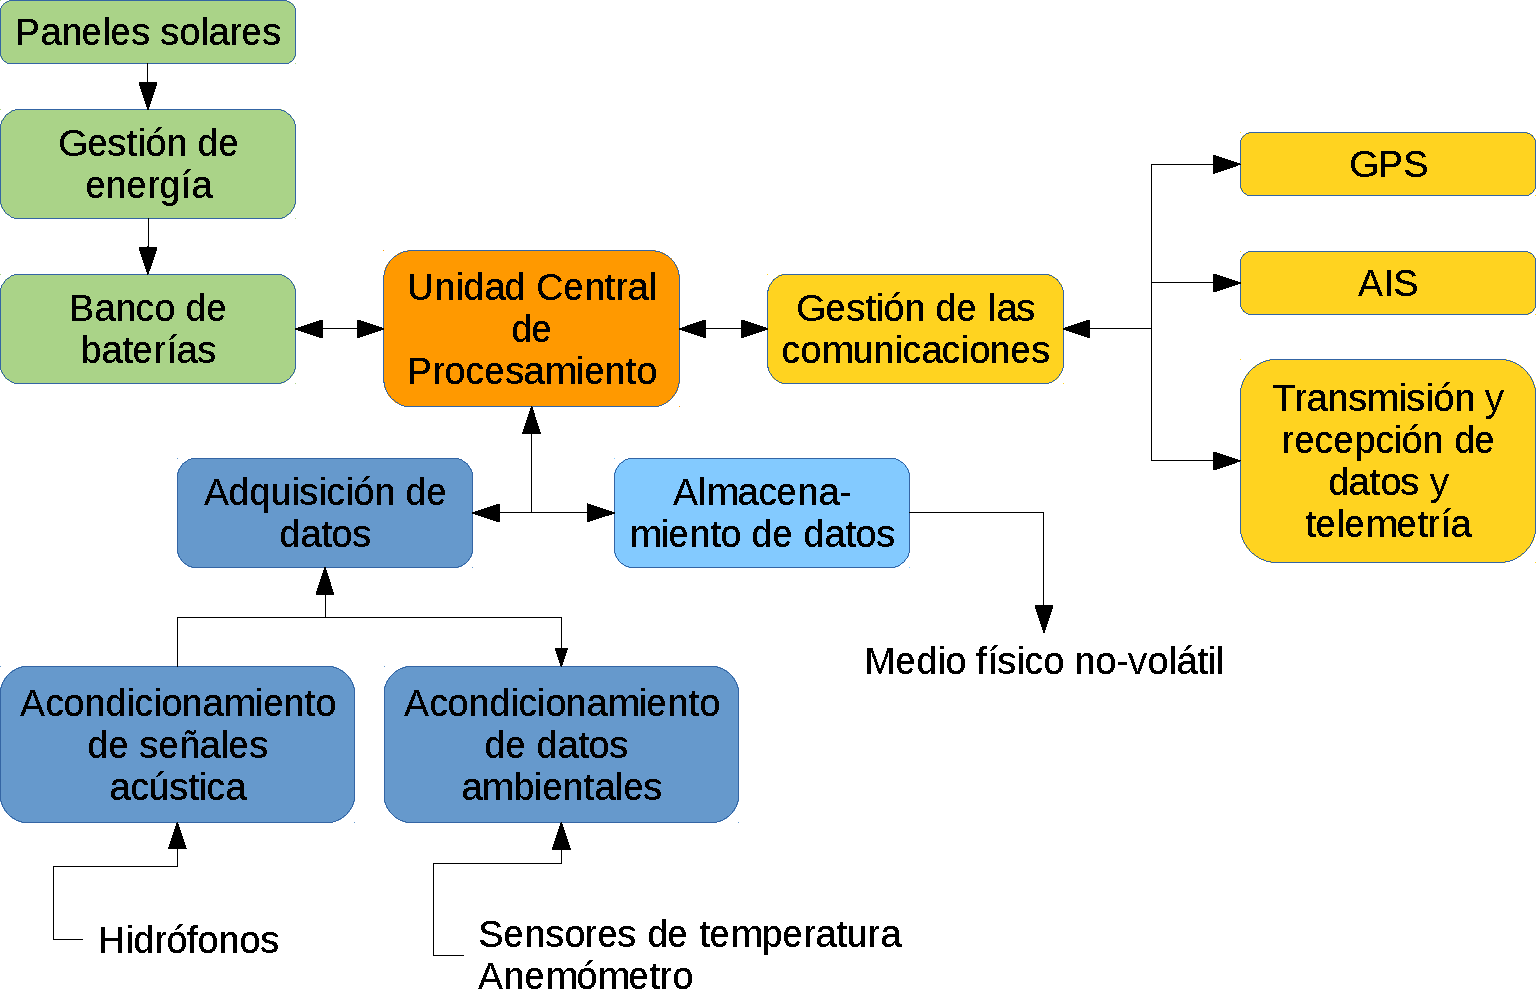
\includegraphics[width=\textwidth]{./Figures/Diagrama_en_Bloques.pdf}
	\caption[Diagrama en bloques del sistema.]{Diagrama en bloques del sistema. Se diferencian por color los subsistemas funcionales: energía; unidad central de procesamiento; comunicaciones; adquisición y almacenamiento.}
	\label{fig:diagramaBloques}
\end{figure}

Para alcanzar el objetivo general se dispone de un paquete tecnológico compuesto principalmente por un equipo de trabajo multidisciplinario con conocimientos teóricos de los fenómenos físicos subyacentes a la propagación del sonido en el medio submarino, acceso a bibliografía especializada en acústica submarina y  conocimientos de ingeniería en el campo de los sistemas embebidos.

%Se presenta un diagrama en bloques del sistema en la figura \ref{fig:diagramaBloques} donde se han agrupado por color los distintos sub-módulos que conforman una misma área funcional.

%\begin{figure}
%	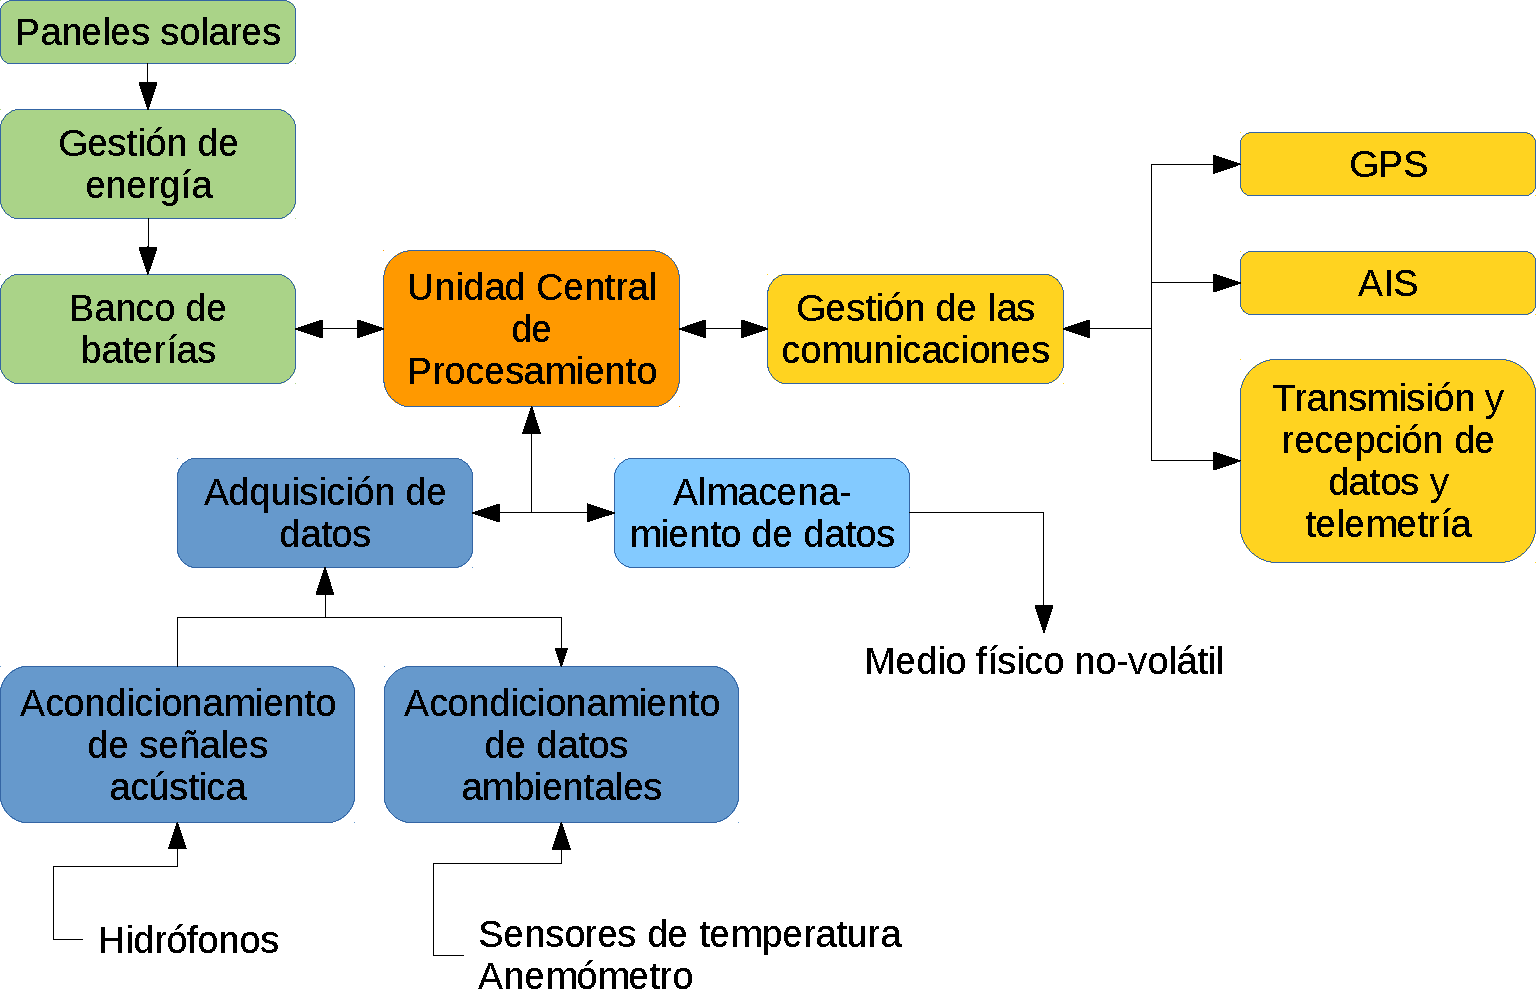
\includegraphics[width=\textwidth]{./Figures/Diagrama_en_Bloques.pdf}
%	\caption{Diagrama en bloques del sistema. Se diferencian por color los distintos sub-módulos funcionales.}
%	\label{fig:diagramaBloques}
%\end{figure}


%----------------------------------------------------------------------------------------

\section{Motivación}

%Para qué sirve medir el ruido submarino.

El conocimiento de valores de NL es fundamental en aplicaciones tales como oceanografía acústica, predicción SONAR, exploración geofísica, comunicación subacuática e ingeniería offshore, entre otras.

Por otra parte, existen muy pocas normas a nivel internacional para la estandarización de la medición in-situ del ruido ambiente subacuático. Si bien en acústica aérea sí existen estándares nacionales e internacionales muy aceptados, éstos no pueden extrapolarse fácilmente a la acústica subacuática dadas las diferentes características físicas del fluido en el cual se propaga el sonido, respectivamente.

Actualmente, en el ámbito de la comunidad científica internacional existe una creciente necesidad de medición y monitoreo del ruido subacuático. El interés está parcialmente motivado por un marco regulatorio internacional en lo concerniente al impacto ambiental del ruido subacuático de origen antrópico y principalmente para la evaluación de los efectos sobre la vida marina.


%----------------------------------------------------------------------------------------

\section{Objetivos y alcance}

%Objetivo del proyecto, recorte en el alcance

En particular, para el trabajo final de la Maestría en Sistemas Embebidos, se realizará una primera iteración sobre el ciclo de diseño centrada en la programación del sistema embebido que constituye la unidad central de procesamiento de la boya.  Se propone desarrollar sobre la plataforma CIAA-NXP, un firmware multicore de control que utilice ambos procesadores del microcontrolador LPC4337 y sea capaz de cumplir las siguientes funciones:

\begin{itemize}
	\item Adquirir datos ambientales de temperatura y velocidad de viento.
	\item Controlar el sistema mediante una interfaz serie.
	\item Almacenar los datos en una memoria no volátil.
\end{itemize}

En la primera iteración, se contempla la posibilidad de simular algún elemento del sistema según sea necesario para avanzar rápidamente en el diseño del firmware de control y las funciones mencionadas. 

A los fines prácticos de cumplir los requerimientos de tiempo del trabajo final de maestría, quedarán excluídos del diseño:

\begin{itemize}
	\item La transmisión de datos en tiempo real a una estación receptora en tierra.
	\item Consideraciones mecánicas del proyecto.
	\item La gestión de energía.
	\item La gestión y control del señalamiento reglamentario marítimo.
	\item La adquisición de señales acústicas.
\end{itemize}

Según un estudio preliminar, para el registro de señales acústicas resulta necesario una placa de adquisición A/D con características muy específicas en cuanto a frecuencia de muestreo, bits de resolución y figura de ruido, del tipo NI USB-6356\footnote{\url{http://www.ni.com/pdf/manuals/374452c.pdf}} o equivalente.  Este tipo de placas poseen \textit{drivers} propietarios cerrados que, en principio, no fue posible utilizar con la CIAA-NXP.   Por este motivo, la adquisición de señales acústicas también queda excluida del alcance en esta primera iteración.

Se muestra en la figura \ref{fig:diagramaBloquesReducido} un diagrama en bloques reducido con los componentes del sistema incluídos en la presente memoria.

\begin{figure}[h]
  \centering
	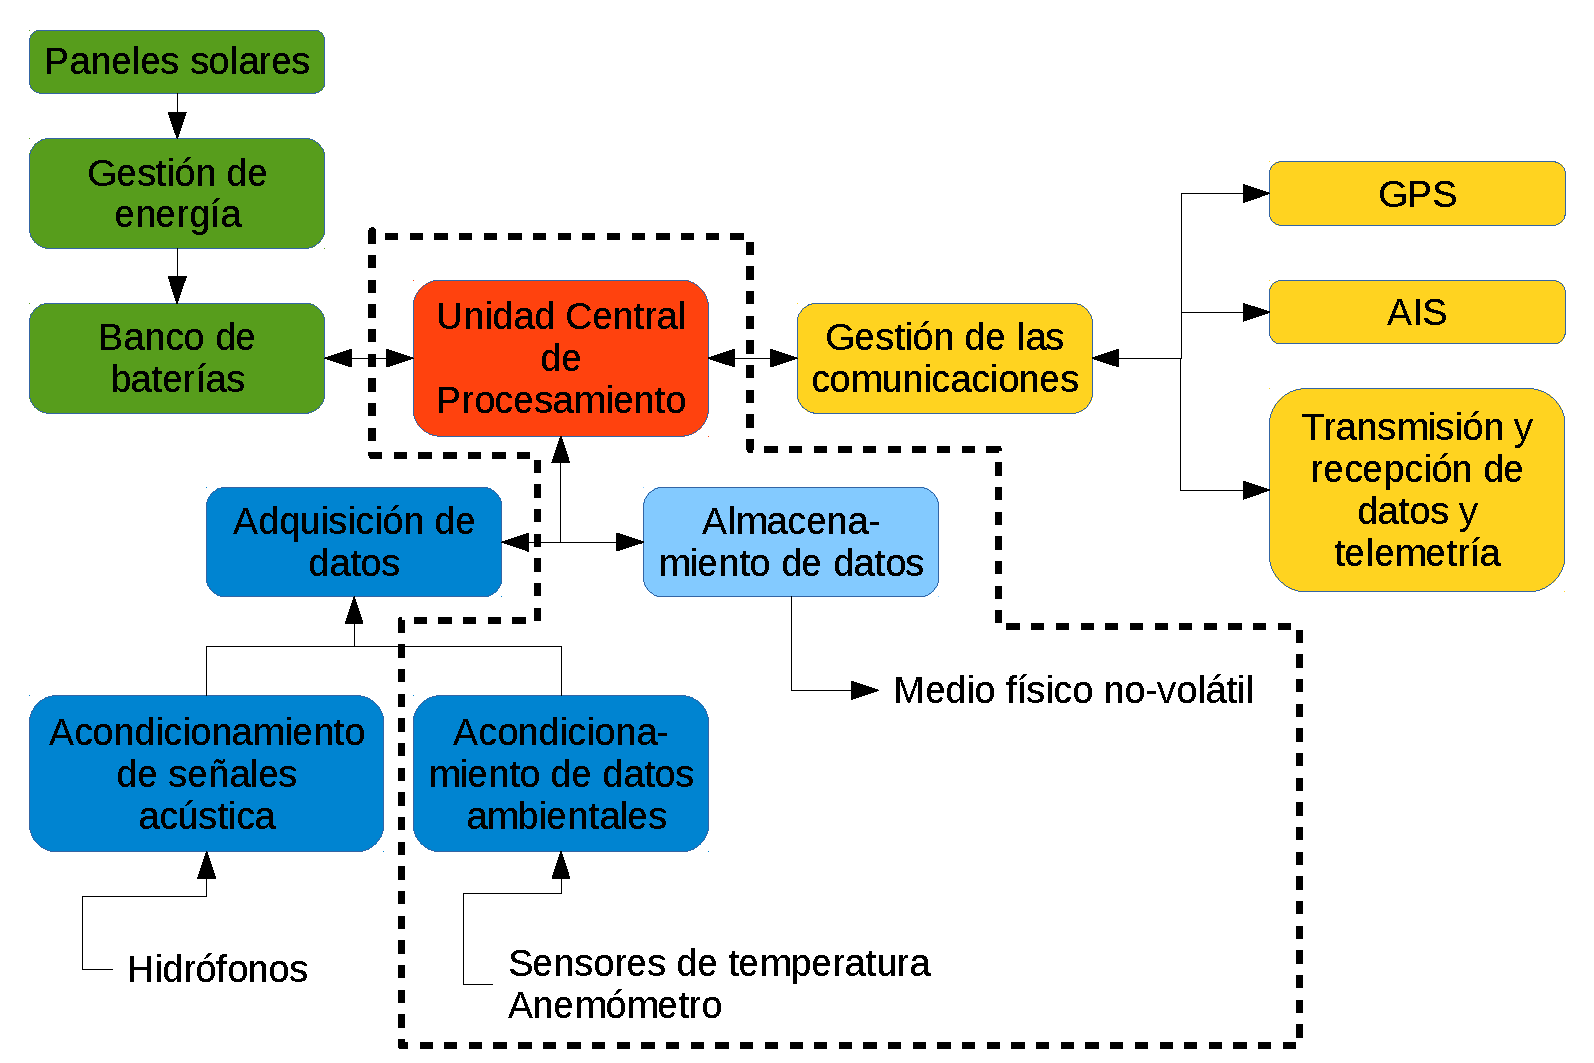
\includegraphics[width=\textwidth]{./Figures/Diagrama_en_Bloques_reducido.pdf}
	\caption{Diagrama en bloques del sistema. Se diferencian por color los distintos sub-módulos funcionales y se indica mediante línea de puntos los componentes incluidos en el alcance.}
	\label{fig:diagramaBloquesReducido}
\end{figure}

%----------------------------------------------------------------------------------------




